\documentclass{article}
\usepackage{graphicx} 
\usepackage{geometry}
\geometry{left=1in, right=1in, top=1in, bottom=1in}
\usepackage{amsfonts}
\usepackage{amsmath}
\usepackage{float}
\usepackage{minted}
\title{CS 6643 HW1}
\author{qgao67@gatech.edu Qidian Gao}
\date{January 17th 2024}

\begin{document}

\maketitle
\textbf{Coworkers:} Me, Yihang Chen and Chatgpt, which is used to optimize the Julia code structure since I'm not familiar with it before.
\section{Part A(a)}
Suppose \(a_1, a_2, a_3, a_4 \in \mathbb{F}\) satisfy the equation
\[
a_1(\boldsymbol{v}_1 + \boldsymbol{v}_2) + a_2(\boldsymbol{v}_2 + \boldsymbol{v}_3) + a_3(\boldsymbol{v}_3 + \boldsymbol{v}_4) + a_4\boldsymbol{v}_4 = 0.
\]
Rearranging the terms algebraically, we get
\[
a_1\boldsymbol{v}_1 + (a_1 + a_2)\boldsymbol{v}_2 + (a_2 + a_3)\boldsymbol{v}_3 + (a_3 + a_4)\boldsymbol{v}_4 = 0.
\]
Given that \(\boldsymbol{v}_1, \boldsymbol{v}_2, \boldsymbol{v}_3, \boldsymbol{v}_4\) are linearly independent, we deduce that
\[
a_1 = 0, a_1 + a_2 = 0, a_2 + a_3 = 0, a_3 + a_4 = 0.
\]
This implies that \(a_2 = 0\), \(a_3 = 0\), and \(a_4 = 0\). Therefore, \(\boldsymbol{v}_1 + \boldsymbol{v}_2, \boldsymbol{v}_2 + \boldsymbol{v}_3, \boldsymbol{v}_3 + \boldsymbol{v}_4, \boldsymbol{v}_4\) are linearly independent.

Next, we show that these vectors span \(V\). Any vector \(\boldsymbol{v} \in V\) can be expressed as
\[
\boldsymbol{v} = a_1\boldsymbol{v}_1 + a_2\boldsymbol{v}_2 + a_3\boldsymbol{v}_3 + a_4\boldsymbol{v}_4.
\]
Each \(\boldsymbol{v}_i\) can be represented in terms of our new vectors as follows:
\[
\begin{aligned}
\boldsymbol{v}_1 &= (\boldsymbol{v}_1 + \boldsymbol{v}_2) - (\boldsymbol{v}_2 + \boldsymbol{v}_3) - (\boldsymbol{v}_3 + \boldsymbol{v}_4) - \boldsymbol{v}_4, \\
\boldsymbol{v}_2 &= (\boldsymbol{v}_2 + \boldsymbol{v}_3) - (\boldsymbol{v}_3 + \boldsymbol{v}_4) - \boldsymbol{v}_4, \\
\boldsymbol{v}_3 &= (\boldsymbol{v}_3 + \boldsymbol{v}_4) - \boldsymbol{v}_4.
\end{aligned}
\]
Therefore,
\[
\begin{aligned}
\boldsymbol{v} &= a_1\boldsymbol{v}_1 + a_2\boldsymbol{v}_2 + a_3\boldsymbol{v}_3 + a_4\boldsymbol{v}_4 \\
&= a_1((\boldsymbol{v}_1 + \boldsymbol{v}_2) - (\boldsymbol{v}_2 + \boldsymbol{v}_3) - (\boldsymbol{v}_3 + \boldsymbol{v}_4) - \boldsymbol{v}_4) \\
&\quad + a_2((\boldsymbol{v}_2 + \boldsymbol{v}_3) - (\boldsymbol{v}_3 + \boldsymbol{v}_4) - \boldsymbol{v}_4) \\
&\quad + a_3((\boldsymbol{v}_3 + \boldsymbol{v}_4) - \boldsymbol{v}_4) + a_4\boldsymbol{v}_4 \\
&= a_1(\boldsymbol{v}_1 + \boldsymbol{v}_2) + (-a_1 + a_2)(\boldsymbol{v}_2 + \boldsymbol{v}_3) \\
&\quad + (-a_1 - a_2 + a_3)\boldsymbol{v}_3 + (-a_1 - a_2 - a_3 + a_4)\boldsymbol{v}_4.
\end{aligned}
\]
Since \(a_1, -a_1 + a_2, -a_1 - a_2 + a_3, -a_1 - a_2 - a_3 + a_4 \in \mathbb{F}\), the set \(\boldsymbol{v}_1 + \boldsymbol{v}_2, \boldsymbol{v}_2 + \boldsymbol{v}_3, \boldsymbol{v}_3 + \boldsymbol{v}_4, \boldsymbol{v}_4\) spans \(V\). Therefore, these vectors form a basis of \(V\).

\section{Part A(b)}
Suppose $\operatorname{dim} U=\operatorname{dim} V=n$. Let $u_1, \ldots, u_n$ be a basis of $U$. Since $U$ is a subspace of $V, u_1, \ldots, u_n$ is linearly independent in $V$ and thus can be extended to a basis of $V$. However, since $u_1, \ldots, u_n$ already contains $n$ vectors, there is nothing to add, hence it is already a basis of $V$. Since $U$ and $V$ share the same basis, $U=V$.

\section{Part A(c)}

Consider a subspace \(A\) of \(\mathbb{R}^3\). By definition, the zero vector is always an element of \(A\). If \(A\) contains only the zero vector, it is the zero subspace of \(\mathbb{R}^3\).

Assume \(A\) contains more than one element, including a non-zero vector \(\boldsymbol{v}\). Since \(A\) is a subspace, it must contain all scalar multiples of \(\boldsymbol{v}\), forming a line through the origin. Suppose \(A\) also contains another distinct point \(\boldsymbol{w}\) not on this line. Our goal is to demonstrate that \(A\) contains the entire plane defined by \(\boldsymbol{v}\) and \(\boldsymbol{w}\). We assert there exist scalars \(a, b \in \mathbb{R}\) such that
\[
a\boldsymbol{v} + b\boldsymbol{w} = \boldsymbol{x},
\]
for any \(\boldsymbol{x}\) in \(\mathbb{R}^3\). The system
\[
\begin{aligned}
a\boldsymbol{v} + b\boldsymbol{w} &= \boldsymbol{x} \\
\end{aligned}
\]
can be solved given that \(\boldsymbol{v}\) and \(\boldsymbol{w}\) are linearly independent. Thus, \(\boldsymbol{x}\) is a linear combination of \(\boldsymbol{v}\) and \(\boldsymbol{w}\), and \(A\) is a subspace.

Since \(\boldsymbol{v}\) and \(\boldsymbol{w}\) are not linearly dependent, the above system has a unique solution. This implies that any vector in \(\mathbb{R}^3\) can be expressed as a linear combination of vectors in \(A\), confirming that \(A\) is a subspace.

We conclude that all subspaces of \(\mathbb{R}^3\) over \(\mathbb{R}\) are either the zero subspace, lines through the origin, planes through the origin, or \(\mathbb{R}^3\) itself.

Consider a subspace \(\mathrm{A}\) of \(\mathbb{R}^3\). By its definition as a subspace, the zero vector \((0,0,0)\) must be a member of \(\mathrm{A}\). If \(\mathrm{A}\) contains only this zero vector, it is identified as the trivial subspace of \(\mathbb{R}^3\).

Suppose \(\mathrm{A}\) includes more elements beyond the zero vector, such as a non-zero vector \(\mathrm{s} = (x_0, y_0, z_0)\). Given that \(\mathrm{A}\) is a subspace, for any scalar \(\alpha \in \mathbb{R}\), the vector \(\alpha \mathrm{s}\) belongs to \(\mathrm{A}\). Thus, \(\mathrm{A}\) encompasses the line connecting the origin with \(\mathrm{s}\). 

If this line is a subset of \(\mathrm{A}\), then \(\mathrm{A}\) must also contain a distinct point \(\mathrm{t} = (x_1, y_1, z_1)\), which is not a scalar multiple of \(\mathrm{s}\). Our aim is to show that every vector in \(\mathbb{R}^3\) is a member of \(\mathrm{A}\). 

For any vector \((a, b, c) \in \mathbb{R}^3\), we posit the existence of scalars \(\alpha, \beta, \gamma \in \mathbb{R}\) satisfying:
\[
(a, b, c) = \alpha \mathrm{s} + \beta \mathrm{t} + \gamma \mathrm{r}.
\]
This is confirmed by solving the system:
\[
\begin{aligned}
a &= \alpha x_0 + \beta x_1 + \gamma x_2, \\
b &= \alpha y_0 + \beta y_1 + \gamma y_2.
\end{aligned}
\]

Given that \(\mathrm{s}, \mathrm{t}, \mathrm{r}\) are not linearly dependent, the above system yields a unique solution. Therefore, the vector \((a, b, c)\) is a linear combination of \(\mathrm{s}, \mathrm{t}, \mathrm{r}\) in \(\mathrm{A}\), affirming that \(\mathrm{A}\) is indeed a subspace of \(\mathbb{R}^3\).
All subspaces of \(\mathbb{R}^3\) over \(\mathbb{R}\) are classified as the zero subspace, lines through the origin, planes through the origin, or the entirety of \(\mathbb{R}^3\) itself.
\section{Part B}
\subsection{Inequality 1}
\textbf{Statement:} 
\[
\| \boldsymbol{x} \|_{\infty} \leq \| \boldsymbol{x} \|_2 \leq \sqrt{n} \| \boldsymbol{x} \|_{\infty}.
\]

\textbf{Proof:} 
The infinity norm \(\| \boldsymbol{x} \|_{\infty}\) is defined as \(\max_i |x_i|\), and the 2-norm \(\| \boldsymbol{x} \|_2\) as \(\sqrt{\sum_{i=1}^n x_i^2}\).

\textit{Left inequality:} Given \(|x_i| \leq \max_i |x_i|\) for all \(i\), it follows that
\[
\| \boldsymbol{x} \|_2 = \sqrt{\sum_{i=1}^n x_i^2} \geq \sqrt{\max_i |x_i|^2} = \| \boldsymbol{x} \|_{\infty}.
\]

\textit{Right inequality:} Since each \(|x_i|^2 \leq \max_i |x_i|^2\), we have
\[
\| \boldsymbol{x} \|_2 = \sqrt{\sum_{i=1}^n x_i^2} \leq \sqrt{n \max_i |x_i|^2} = \sqrt{n} \| \boldsymbol{x} \|_{\infty}.
\]
\subsection{Inequality 2}
Let $x \in \mathbb{R}_{\infty}^n$. We know that $\|y\|_{\infty} \leq\|y\|_2 \leq \sqrt{n}\|y\|_{\infty}$ for all $y \in \mathbb{R}^n$, so
$$
\|A(x)\|_{\infty} \leq\|A(x)\|_2 \leq\|A\|_2\|x\|_2 \leq\|A\|_2 \sqrt{n}\|x\|_{\infty}
$$

Since $x \in \mathbb{R}_{\infty}^n$ is arbitrary
$$
\|A\|_{\infty} \leq \sqrt{n}\|A\|_2
$$
\subsection{Inequality 3}
Let $\mathrm{A}$ be some square $\mathrm{n}$ by $\mathrm{n}$ matrix.

Let $\vec{x}=\left(x_1, x_2, \ldots, x_n\right)^T$ where $x \in \mathbb{R}$ and $n \in \mathbb{N}^{+}$
We want to prove that $\|A\|_2 \leq \sqrt{n}\|A\|_{\infty}$
Now we know that $\|A\|_p \equiv\|A \vec{x}\|_p /\|\vec{x}\|_p$
Then the inequality becomes: $\|A \vec{x}\|_2 /\|\vec{x}\|_2 \leq \sqrt{n}\|A \vec{x}\|_{\infty} /\|\vec{x}\|_{\infty}$
So lets look at the top:
$$
\|A \vec{x}\|_2 \leq \sqrt{n}\|A \vec{x}\|_{\infty}
$$

Screw root signs:
$$
\begin{aligned}
& \left(\|A \vec{x}\|_2 \leq \sqrt{n}\|A \vec{x}\|_{\infty}\right)^2 \\
& \|A \vec{x}\|_2^2 \leq n\|A \vec{x}\|_{\infty}^2
\end{aligned}
$$

Let $A \vec{x}=\vec{b}$ since a matrix times a vector is a vector.

We also know that:
$$
\|\vec{b}\|_2 \equiv \sqrt{\Sigma\left(x_1^2+x_2^2+\ldots x_n^2\right)}
$$

Thus $\|\vec{b}\|_2^2 \equiv \Sigma\left(x_1^2+x_2^2+\ldots x_n^2\right)$
Consider the definition of the infinity norm of a vector \(\vec{b}\), which is given by:
$$
\|\vec{b}\|_{\infty} = \max \{|x_k| : 1 \leq k \leq n\}.
$$

This leads to the following inequality:
$$
\sum_{i=1}^{n} x_i^2 \leq n \left(\max_{1 \leq k \leq n} |x_k|\right)^2.
$$

The rationale behind this inequality is straightforward: the sum of the squares of all elements in vector \(\vec{x}\) will never exceed the square of its largest element, multiplied by \(n\). However, a point of confusion arises when considering the relationship between the 2-norm and the infinity norm of \(\vec{x}\). We 
can use somewhat unusual way, stating that:
$$
\|\vec{x}\|_2 \geq \|\vec{x}\|_{\infty}.
$$

This inequality initially seemed counterintuitive, where it appeared more like a comparison:
$$
\frac{\|A \vec{x}\|_2 \leq \|A \vec{x}\|_{\infty}}{\|\vec{x}\|_2 \geq \|\vec{x}\|_{\infty}}.
$$

Note that the division line here is simply a representation of the attempt to articulate the concept via MathJax. Nevertheless, understanding that \(\|\vec{x}\|_2 \geq \|\vec{x}\|_{\infty}\) is indeed correct, we can assert, based on the properties of inequalities, that the following holds:
Consider the following inequality:
\[
\frac{1}{\|\vec{x}\|_2} \leq \frac{1}{\|\vec{x}\|_{\infty}}.
\]
This is where the inversion of the inequality sign becomes apparent. Given that it is established that \(\|\vec{x}\|_2 \geq \|\vec{x}\|_{\infty}\), and considering that the right-hand side (RHS) is likely to be greater than or equal to the left-hand side (LHS), dividing both sides by 1 results in the LHS becoming the smaller quantity.\par
Therefore, it logically follows that:
\[
\|A\|_2 \leq \sqrt{n}\|A\|_{\infty}.
\]



\section{Part C(a)}
Let $u, v \in e^n$. Let $A=I+u v^*$
(1) Let $A$ is invertible. Then $A^{-1}$ exists.
$$
\begin{aligned}
& \text { Let } B=u v^*, \omega=v^* u \\
& (I+B)\left(I-\frac{1}{1+\omega} B\right) \\
& =\frac{1}{(1+w)}(I+B)(I-B+\omega I) \\
& =\frac{1}{(1+\omega)}\left(I-B^2+\omega I+\omega B\right) \\
& =\frac{1}{(1+\omega)}[I(1+\omega)+B(\omega I-B)] \\
& B^2=\left(u v^*\right)\left(u v^*\right)=u\left(v^* u\right) v^*=u \omega v^* \omega u v^*=\omega B \\
& B(\omega I-B)=B \omega I-B^2=\omega B-B^2=\omega B-\omega B=0
\end{aligned}
$$
from (1), (2) we get
$$
(I+B)\left(I-\frac{1}{1+\omega} B\right)=\frac{1}{(1+\omega)}[I(1+\omega)+0]=I
$$

Hence $(I+B)^{-1}=I-\frac{1}{(1+\omega)} B$
$$
r_1\left(I+u v^*\right)^{-1}=I-\frac{1}{\left(1+v^* u\right)} u v^*
$$
where $\alpha=-\frac{1}{\left(1+v^* u\right)} \in C$
Hence if $A$ is invertible, $\exists \alpha \in C$ sit $A_{=}^{-1} I+\alpha u v^*$
\section{Part C(b) and (c)}
If $A$ is singular then Null $(A)=\operatorname{span}\{u\}, n \neq 0$ $A(k u)=0$ for any $k \in C . \Rightarrow\left(k+k\left(v^* u\right)\right) u=0$
$$
\Rightarrow v^* u=-1
$$
$\operatorname{det}(A)=1+v^* u . A$ is singular $\Leftrightarrow \operatorname{det}(A)=0$
$$
\Leftrightarrow v^* u=-1
$$

To find $\operatorname{mull}(A)$. Set $A x=0$ for some $m$-vectors $x$. (I tu*) $x=0 \Rightarrow u k^* x=-x$. Since $v^* u=-1$ we get $x=u \cdot \operatorname{mull}(A)=\operatorname{span}\{u\}$.
\section{Julia}
First, I successfully launched the HW code in Julia:
\begin{figure}[H]
  \centering
  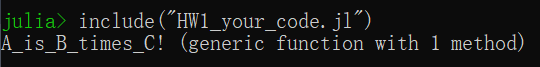
\includegraphics[width=0.5\textwidth]{1.png}
  \label{fig:image_label}
\end{figure}
Then I tested on cmd using the driver file:
\begin{figure}[H]
  \centering
  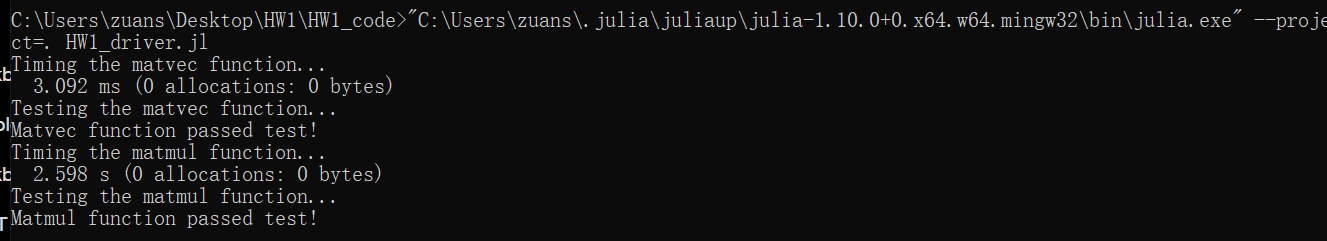
\includegraphics[width=0.5\textwidth]{2.png}
  \label{fig:image_label}
\end{figure}
I used the following code to optimize the result:
\begin{minted}{Julia}
using BenchmarkTools
@btime A_is_B_times_C!(A, B, C)
\end{minted}
\begin{figure}[H]
  \centering
  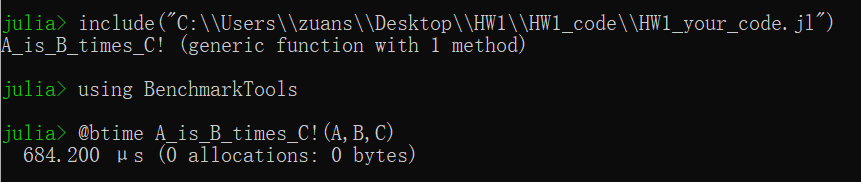
\includegraphics[width=0.5\textwidth]{3.png}
  \label{fig:image_label}
\end{figure}
\end{document}
